\documentclass[12pt%
%,draft%
,aspectratio=169%
]{beamer}
%
\usepackage{fontspec}
\defaultfontfeatures{Ligatures=TeX}
%\setsansfont{Liberation Sans}
\usepackage{polyglossia}
\setdefaultlanguage{ngerman}
% Alternative template for talks of the Freie Universität Berlin.
% Created by Leonard R. König, <leonard.koenig@fu-berlin.de> following the
% guidelines on www.fu-berlin.de/cd
%
% (c) Leonard König, CC BY 4.0
%
% This template was written against UTF-8 capable LaTeX engines, specifically
% LuaLaTeX.

% Trying to get rather close to the ppt/odp template:
%  http://www.fu-berlin.de/sites/cd/downloads_container/PowerPoint_Praesentation_Anleitung.pdf

%%% font styles
\setbeamerfont{frametitle}{series=\bfseries}
\setbeamerfont{footline}{series=\bfseries}
\setbeamerfont{headline}{series=\bfseries}
\setbeamerfont{alerted text}{series=\bfseries}
%%%

% colordefs
\definecolor{fu_darkblue}{RGB}{0,51,102}
\definecolor{fu_seablue}{RGB}{0,102,204}
\definecolor{fu_lightblue}{RGB}{204,214,224}
\definecolor{fu_green}{RGB}{153,204,0}
\definecolor{fu_lightgrey}{RGB}{128,128,128}
\definecolor{fu_grey}{RGB}{95,95,95}
%
\definecolor{fu_red}{RGB}{204, 0, 0} % red text (used by \alert)
%%% end colordefs

%%% colors
\setbeamercolor*{title}{fg=fu_darkblue}
\setbeamercolor*{subtitle}{fg=fu_seablue}
\setbeamercolor*{frametitle}{fg=fu_darkblue}
\setbeamercolor*{footline}{fg=fu_grey,bg=fu_lightblue}
\setbeamercolor*{headline}{fg=fu_grey}

\setbeamercolor*{normal text}{fg=black}
\setbeamercolor*{alerted text}{fg=fu_red}
\setbeamercolor*{example text}{fg=fu_green}
\setbeamercolor*{structure}{fg=fu_darkblue}

\setbeamercolor*{block title}{fg=white,bg=black!50}
\setbeamercolor*{block title alerted}{fg=white,bg=black!50}
\setbeamercolor*{block title example}{fg=white,bg=black!50}

\setbeamercolor*{block body}{bg=black!10}
\setbeamercolor*{block body alerted}{bg=black!10}
\setbeamercolor*{block body example}{bg=black!10}

\setbeamercolor{bibliography entry author}{fg=fu_darkblue}

\setbeamercolor{item}{fg=fu_darkblue}
\setbeamercolor{navigation symbols}{fg=fu_lightgrey,bg=fu_grey}
%%% end colors

%%% title page
% Display logo (if exists) and right next to it, put our title + subtitle
\defbeamertemplate*{title page}{fu_titlepage}
{%
	\hskip .3\textheight
	\begin{minipage}[.4\textheight]{\textwidth}
		\begin{minipage}[.4\textheight]{0.25\textwidth}
			\inserttitlegraphic
		\end{minipage}%
		\begin{minipage}[.4\textheight]{0.75\textwidth}
			\begin{beamercolorbox}{title}
				\usebeamerfont{title}\inserttitle\par%
			\end{beamercolorbox}
			\vfill
			\ifx\insertsubtitle
				\@empty%
			\else
				\begin{beamercolorbox}{subtitle}
					\usebeamerfont{subtitle}\insertsubtitle\par
				\end{beamercolorbox}
			\fi
		\end{minipage}
	\end{minipage}%
	\hskip .3\textheight
}
%%% end title page

%%% headline
% display title, author and institute on the left;
% logo on the right.
\newcommand{\headlinetext}
{%
	\inserttitle\\[0.3em]%
	\insertauthor, %
	\insertshortinstitute
}
\newlength{\headlinewidth}
\setlength{\headlinewidth}{\paperwidth}
\addtolength{\headlinewidth}{-2\marginparsep}
\setbeamertemplate{headline}
{%
	\begin{beamercolorbox}[wd=\paperwidth]{headline}%
		\vskip5pt
		{\hspace*{\marginparsep}}%
		\parbox{.5\headlinewidth}
		{%
			\usebeamertemplate{title in head/foot}%
			\headlinetext%
		}%
		\begin{minipage}{.5\headlinewidth}%
			\hfill\usebeamertemplate*{logo}
		\end{minipage}%
		{\hspace*{\marginparsep}}%
	\end{beamercolorbox}%
}
%%% end headline

%%% footline
% title + date on the left, frame number on the right
\newcommand{\footlinetext}
{%
	\usebeamerfont{shorttitle}\insertshorttitle, %
	\usebeamerfont{shortdate}\insertshortdate
}
\setbeamertemplate{footline}
{%
	\begin{beamercolorbox}{footline}
		\vskip2pt
		\hspace{\marginparsep}%
		\footlinetext\hfill%
		\insertframenumber%
		\hspace{\marginparsep}
		\vskip2pt
	\end{beamercolorbox}%
}
%%% end footline

% don't use default templates for sidebars
\setbeamertemplate{sidebar right}{}
\setbeamertemplate{sidebar left}{}
\setbeamertemplate{title page}[fu_titlepage]
\usepackage{amsmath}
\usepackage{amsfonts}
\usepackage{amssymb}
\usepackage{graphicx}
\usepackage{algorithm}
\usepackage[noend]{algpseudocode}
%\usepackage{algorithmic}
\usepackage{tikz}
\usetikzlibrary{arrows,shapes,automata,petri,positioning,calc}
\usepackage{graphicx}
\usepackage{subfig}
\usepackage{pgfplots}
\usepackage{venndiagram}
\usepackage{ stmaryrd }
\usepackage{circuitikz}
\usepackage{bohr}
\usepackage{csquotes}


\usepackage{luacode} % for '\luaexec' macro
%% Define a LaTeX "wrapper" macro:
\newcommand\bitwiseXOR[2]{\luaexec{tex.sprint((#1)~(#2))}}
\newcommand\bitwiseAND[2]{\luaexec{tex.sprint((#1)&(#2))}}
\newcommand\bitwiseOR[2]{\luaexec{tex.sprint((#1)|(#2))}}


\def\CalcC#1{%
\coordinate (base) at (#1.B);
\coordinate (collector) at (#1.C);
\coordinate (emitter) at (#1.E);
\draw (barycentric cs:base=0.32,collector=0.5,emitter=0.5) circle [radius=14pt];
}

\pgfplotsset{
    standard/.style={%Axis format configuration
        axis x line=middle,
        axis y line=middle,
        enlarge x limits=0.15,
        enlarge y limits=0.15,
        every axis x label/.style={at={(current axis.right of origin)},anchor=north west},
        every axis y label/.style={at={(current axis.above origin)},anchor=north east},
        every axis plot post/.style={mark options={fill=white}}
        }
    }


\author{Benjamin Tröster}
\title[Schalttechnik \& Logikgatter]{Schalttechnik}
%\subtitle[Markov Models]{...}
%\pgfdeclareimage{titlegraphic}{../res/dwarf_logo2.png}
%\titlegraphic{\pgfuseimage{titlegraphic}}
%\date{}
%\subject{}
%
% FU settings
\institute[HTW Berlin]{Hochschule für Technik und Wirtschaft Berlin}
%\pgfdeclareimage[height=0.9cm]{logo}{../res/dwarf_logo}
%\logo{\pgfuseimage{logo}}
%
\usepackage[
backend=biber,
citestyle=alphabetic,bibstyle=authoryear
]{biblatex}
\addbibresource{sources.bib}


\begin{document}

\begin{frame}
\titlepage
\end{frame}

\begin{frame}{Fahrplan}
\tableofcontents[hideothersubsections]
\end{frame}

\section{Chip-Fertigung}

\subsection{Überblick}

\begin{frame}{Überblick}
\begin{columns}[T] % align columns
\begin{column}{.58\textwidth}
\begin{itemize}
	\item Ausgangsmaterial ist Quarzsand
	\item Hier drin ist Silizium (Siliziumdioxid) enthalten
	\item Quarzsand $\to$ Siliziumschmelze
	\item Es entsteht ein Einkristall -- Ingot
	\item Ingot in $0,5$ -- $1,5 mm$ dünne Scheiben (Wafer)
	\item Anschließend Polieren des Wafers $\to$ Unebenheiten entfernen
	\item Aufbringen der Transistoren, Leiter und Isolatoren $\to$ Planartechnik
	\item $\to$ FOEL (\emph{Front-end of line})
Scheiben zersäg
\end{itemize}
\end{column}%
\hfill%
\begin{column}{.38\textwidth}
\centering
\vspace*{-1cm}
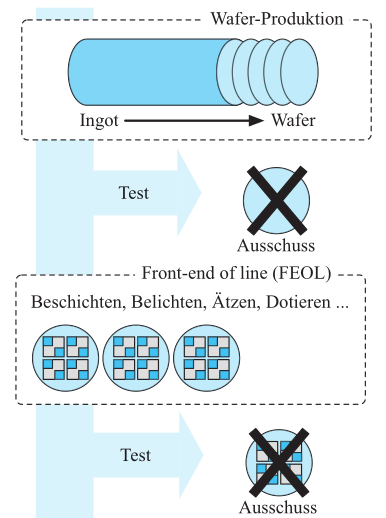
\includegraphics[scale=0.4]{pictures/ic1}
\end{column}%
\end{columns}
\end{frame}

\begin{frame}{Überblick}
\begin{columns}[T] % align columns
\begin{column}{.58\textwidth}
\begin{itemize}
	\item Verbinden der Anschlüsse der erzeugten Schaltelemente
	\item $\to$ BOEL (\emph{Back-end of line})
	\item Jeder Wafer enthält vollständig ausgebildete, identischer Chip-Kerne $\to$ Dies
	\item Vereinzelung: Wafer $\to$ Spezialfolie (blue tape)
	\item Dicing: Zersägen der Wafer
	\item Packaging: Einsetzen der Chip-Kerne in Gehäuse, interne \& externe Anschlüsse anbringen
\end{itemize}
\end{column}%
\hfill%
\begin{column}{.38\textwidth}
\centering
\vspace*{-1cm}
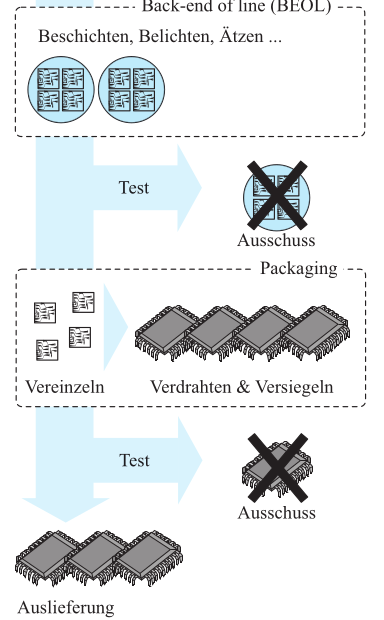
\includegraphics[scale=0.4]{pictures/ic2}
\end{column}%
\end{columns}
\end{frame}

\subsection{Planartechnik}
\begin{frame}{Planartechnik}
\begin{itemize}
	\item Fertigungsmethode in vier Schritten:
	\begin{itemize}
		\item Beschichtungstechnik
		\item Belichtungstechnik
		\item Ätztechnik
		\item Dotierungstechnik
	\end{itemize}
\end{itemize}
\end{frame}

\begin{frame}{Beschichtungstechnik}
\begin{columns}[T] % align columns
\begin{column}{.58\textwidth}
\begin{itemize}
	\item Erhitzung Wafer ca. $1000^\circ C$
	\item Zuleitung von Sauerstoff $\to$ Silizium-Substrats oxidiert
	\item $\to$ isolierenden Schicht überzogen
	\item Spin-Coating-Verfahren: Beschichtung lichtempfindlicher Fotolack
\end{itemize}
\end{column}%
\hfill%
\begin{column}{.38\textwidth}
\centering
\vspace*{-1cm}
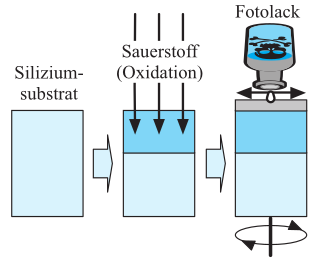
\includegraphics[scale=0.5]{pictures/beschichtung}
\end{column}%
\end{columns}
\end{frame}

\begin{frame}{Belichtungstechnik (Lithografie)}
\begin{columns}[T] % align columns
\begin{column}{.58\textwidth}
\begin{itemize}
	\item Aussetzen des Wafers mit kurzwelligem UV-Licht
	\item Hochfrequenten Strahlen
	\item Spezielle Maske sorgt für partielle Aushärtung
	\item Herauslösung unbelichteten Lackanteile
	\item Freilegung darunterliegenden Oxidstellen
\end{itemize}
\end{column}%
\hfill%
\begin{column}{.38\textwidth}
\centering
\vspace*{-1cm}
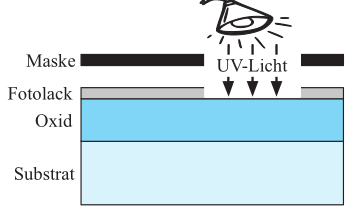
\includegraphics[scale=0.45]{pictures/belichtung}
\end{column}%
\end{columns}
\end{frame}

\begin{frame}{Ätztechnik}
\begin{columns}[T] % align columns
\begin{column}{.58\textwidth}
\begin{itemize}
	\item Tauchbad in Ätzender Flüssigkeit
	\item Lönung greift Halbleiterkristall an freiliegenden Stellen an
	\item Eindringen der lithografisch aufgetragene Muster in die Oxidschicht
	\item Säuberung des Wafers nach Ätzvorgang
\end{itemize}
\end{column}%
\hfill%
\begin{column}{.38\textwidth}
\centering
\vspace*{-1cm}
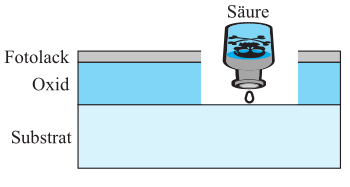
\includegraphics[scale=0.45]{pictures/aetz}
\end{column}%
\end{columns}
\end{frame}

\begin{frame}{Dotierungstechnik}
\begin{columns}[T] % align columns
\begin{column}{.58\textwidth}
\begin{itemize}
	\item Erhitzen des Siliziumkristalls
	\item Versetzen der zugänglichen Stellen des Substrats mit Fremdatomen
	\item Dotierung:
	\begin{itemize}
		\item Dotierung mittels Ionenbeschuss
		\item Diffusion aus einen Dotiergas
		\item Aufbringen eines speziellen Dotierlacks
	\end{itemize}
\end{itemize}
\end{column}%
\hfill%
\begin{column}{.38\textwidth}
\centering
\vspace*{-1cm}
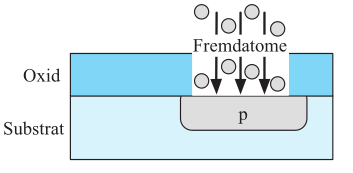
\includegraphics[scale=0.45]{pictures/dotierung}
\end{column}%
\end{columns}
\end{frame}

\subsection{Beispiel: CMOS Inverter}
\begin{frame}{CMOS Inverter}
\begin{columns}[T] % align columns
\begin{column}{.58\textwidth}
\begin{itemize}
	\item CMOS Inverter: Ein Eingangssignal $\to$ Ein Ausgangssignal
	\item Realisiert durch: $n$-Kanal- \& $p$-Kanal-MOSFET
	\item Gate-Anschlüsse angesteuert durch gleiche Spannungsquelle
	\item $p$- \& $n$-MOSFET in Reihe geschaltet
	\item Gesamtschaltung: drei Anschlüsse
\end{itemize}
\end{column}%
\hfill%
\begin{column}{.38\textwidth}
\centering
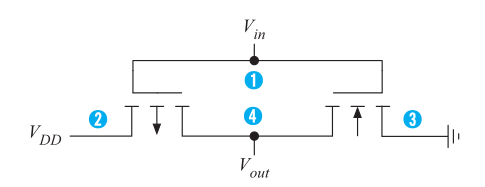
\includegraphics[scale=0.35]{pictures/inverter_shaltung}
\end{column}%
\end{columns}
\end{frame}

\begin{frame}{CMOS Inverter}
\begin{figure}
\center
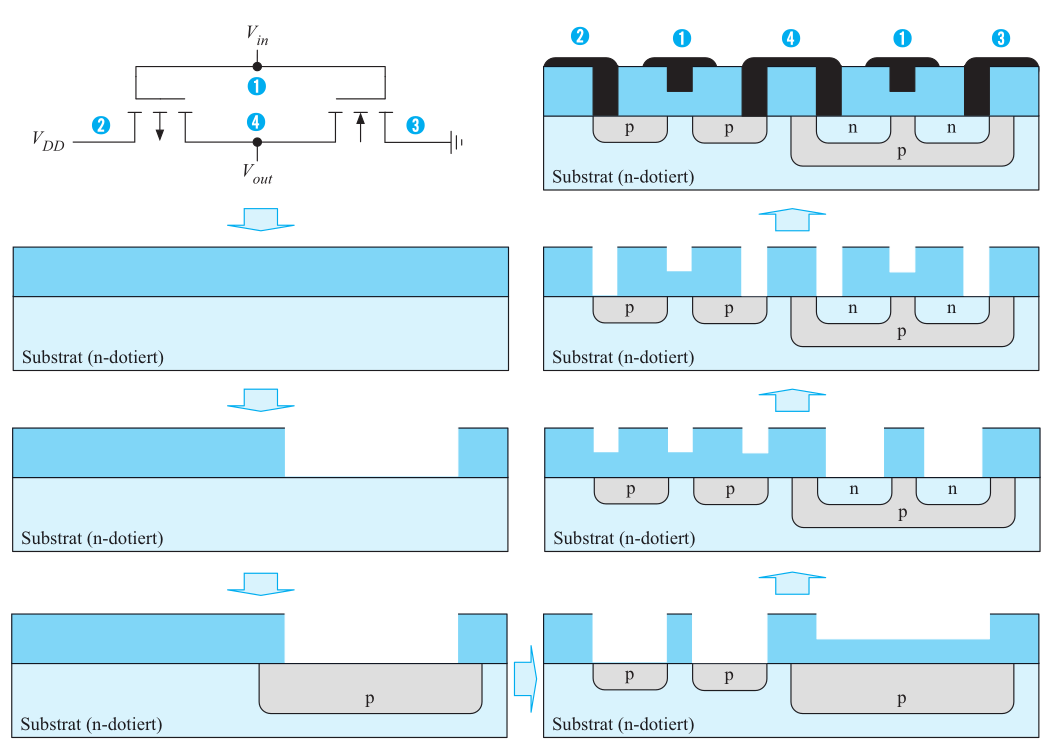
\includegraphics[scale=0.3]{pictures/cmos_inverter}
\caption{Übernommen aus \cite{hoffmann2020grundlagen}.}
\end{figure}
\end{frame}

\begin{frame}{CMOS Inverter}
\begin{itemize}
	\item FEOL $\surd$
	\item Back-end of line?
	\item Verdrahtung fehlt noch!
	\item Im wesentlichen gleiche Techniken, jedoch
	\begin{itemize}
		\item Dotierungstechnik wird ab jetzt nicht mehr benötigt
	\end{itemize}
\end{itemize}
\end{frame}

\begin{frame}{CMOS Inverter, BEOL \& Packaging}
\begin{columns}[T] % align columns
\begin{column}{.58\textwidth}
\begin{itemize}
	\item Auftragen mehrerer Verdrahtungsebenen (Wiring-Layers) aus isolierendem Material
	\item Kanäle für die Leiterbahnen eingeätzt und anschließend der metallische Leiter aufgedampft
	\item Wafer enthält identische Dies $\to$ Packaging
	\item Einsetzen ins Gehäuse, Verbinden interner Anschlüsse mit externer Pins
\end{itemize}
\end{column}%
\hfill%
\begin{column}{.38\textwidth}
\centering
\vspace*{-1cm}
\hspace*{-1cm}
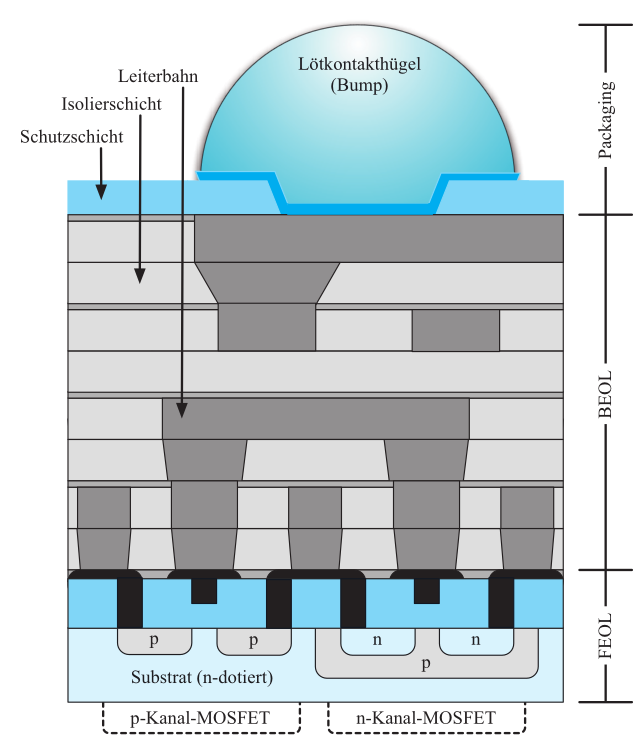
\includegraphics[scale=0.3]{pictures/querschnitt_cmos_inverter}
\end{column}%
\end{columns}
\end{frame}

\section{Integrationsdichte}

\begin{frame}{Integrationsdichte}
\begin{itemize}
	\item Integrationsdichte: Anzahl der Transistoren pro Flächeneinheit auf einem Silizium-Chip
	\item Angabe Integrationsdichte meist als Strukturbreite eines Transistors
	\item Mit Kanallänge identisch $to$ entspricht Abstand zwischen dem Drain- \& Source-Gebiet eines Transistors
	\item Kanallänge verhält sich reziprok zur Integrationsdichte
	\begin{itemize}
		\item Große Kanallängen bedeuten eine niedrige Integrationsdichte
		\item Kleine Kanallängen hohe Integrationsdichte
	\end{itemize}
	\item Ziel: möglichst niedrige Kanallänge
	\begin{itemize}
		\item Verringerung Strukturbreite bedeutet größere Anzahl der Transistoren auf gleichen Fläche
		\item Schaltungen lassen sich kompakter entwerfen
		\item $to$ Kosteneffizienter
		\item Verringerung der Kanallänge führt Erhöhung der Schaltgeschwindigkeit
		\item Verringerung der Leistungsaufnahme $\to$ Stromsparend
	\end{itemize}
\end{itemize}
\end{frame}

\begin{frame}{Integrationsdichte}
\begin{figure}
\center
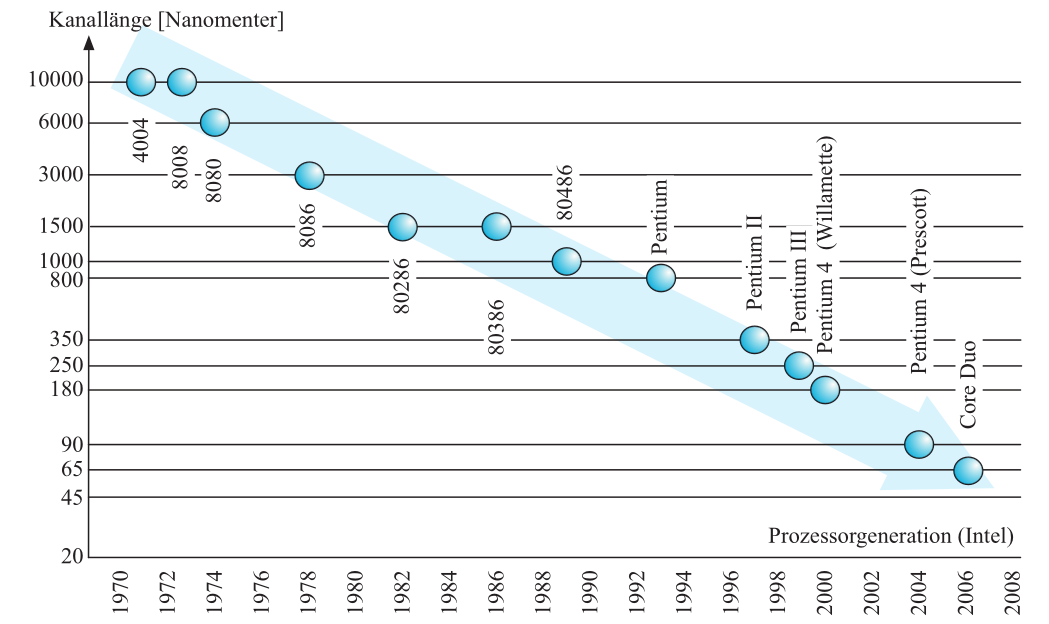
\includegraphics[scale=0.35]{pictures/integrationsdichte}
\caption{Übernommen aus \cite{hoffmann2020grundlagen}.}
\end{figure}
\end{frame}


\section*{Quellen}
\appendix
\begin{frame}[allowframebreaks]
  \frametitle<presentation>{Quellen}
\printbibliography
\end{frame}
\end{document}